\section{Umsetzung}



\subsection{Generierung von Voronoi-Graphen}

\@todo(viktor):{ Erklärung der Generierung separat zur erklärung der Anforderung an den Graphen auf dem der Algorithmus laufen soll \\}
\begin{itemize}
    \item Der Algorithmus arbeitet auf einem gegebenen Graphen. Die Verteilung der Zellen kann regelmäßig oder ohne Struktur sein. Es muss kann auch über den Graphen hinweg variieren. Jede Zelle hat eine 2D Position und jeder Zelle müssen alle ihre Nachbarzellen zugewiesen werden. Zellen sind benachbart, wenn sie eine Kante teilen. Eine Kante sind alle Punkte die gleichweit von zwei Zellenmittelpunkten entfernt sind. 
    \item In meiner Anwendung erstelle ich die Graphen prozedural aus einfachen Mustern oder mittels Zufallsprinzip. 
    \item Meine generierten Graphen sind immer planar, da ich immer dem selben Ablauf folge. Erst erstelle ich eine Menge an 2D Punkten, die wie gesagt eine beliebige Anordnung habe. Dann erstelle ich auf diesen Punkten eine Delaunay-Triangulierung. Das Gegenstück einer solchen Triangulierung ist ein Voronoi-Diagramm. Man findet es in dem man die Eckpunkte der Dreiecke als Mittelpunkte der Voronoizellen nimmt und die Kanten der Dreiecke enden in den Nachbarzellen jeder Zelle. Da Zellen am Rand von diesem Voronoi-Diagramm nach außen unendlich groß sind, begrenzen wir diese Zellen auf eine freigewählte rechteckige Fläche. 
    \item Zu Beginn des Wave Function Collapse werden alle Zellen mit einer Superposition aller möglichen Zustände initialisiert.
\end{itemize}

\at{@incomplete} Warum generieren wir die Graphen und kurz wie und welche Settings gibt einem die App dafür. 
\at{@visual} Beispiele der Generierung

\at{@placement}
Man kann ein regelmäßiges Quadratgitter als eine spezielle Form von Voronoigraph ansehen. Jedes Quadrat kann als eine Voronoizelle angesehen werden, welche genau alle Punkte die am nächsten zu seinem Mittelpunkt enthällt. Die Nachbarn können nun explizit über die Kanten der Voronoizelle gefunden werden. Zuvor waren diese auch implizit durch die Koordinate des Quadrats im Gitter gegeben.

Für den Algorithmus ist diese Unterscheidung egal und er generiert die gleiche Art von Ausgaben ohne weitere Anpassungen. \at{@visual}
Also können wir auch andere Voronoigraphen als Outputgraphen verwenden.

Um einen Voronoigraphen zu generieren nutze ich die Eigenschaft, dass der duale Graph zu jedem Voronoigraph eine Delaunay-Triangulierung ist. Eine Delaunay Triangulierung kann man auf unterschiedlich Weise aus einer beliebigen Point-Cloud, einer Menge an Punkten im 2D Raum, generieren. Dies ist optimal für mich, da ich nun einfach eine Point-Cloud auf beliebige Weise, also mit oder ohne Struktur und so komplex oder simpel wie ich es will, erstellen und aus dieser ein validen Voronoigraph erhalten kann.

\at{@incomplete} Eigenschaften einer Delauney-Triangulierung nennen

Für die Triangulierung habe ich mich ohne tiefere Beweggründe für den Boywer-Watson Algorithmus entschieden. Der Algorithmus generiert die Triangulierung iterativ in dem jeder Punkt nacheinander eingefügt wird und der Graph angepasst wird, so dass es wieder eine Delaunay-Triangulierung ist.
Zur Hilfe erstellen wir ein Superdreieck, welches alle Punkte enthällt. Nun fügen wir einen Punkt ein und prüfen all bisher gefundenen Dreiecke, ob ihr Umkreis diesen Punkt enhällt. Ist der Punkt innerhalb des Umkreises kann das Dreieck nicht zur finalen Triangulierung gehören. Für alle diese Dreieck sammeln wir nun die Kanten. Jede Kante die nur einmal vorkommt ist teil der Hülle dieser Dreiecke, alle anderen Kanten sind innerhalb dieser Hülle, da sich zwei Dreiecke diese teilen. Diese inneren Kanten werden entfernt und für jede Ecke entlang der Hülle wird eine neue Kante zum eingefügten Punkt erstellt.
Am Ende entfernt alle Kanten zur den Eckpunkten des Superdreiecks aus der Triangulierung und erhällt die Delauney-Triagulierung der Point-Cloud.

Aus der Triangulierung erstellen wir das Voronoidiagram indem wir die Eckpunkte als Mittelpunkte der Voronoizellen nehmen. Die Kanten sagen uns welche Zellen benachbart sind. Um die Kanten der Voronoizelle zu finden nehmen wir von alle Dreiecke in denen der Punkt liegt den Mittelpunkt des Umkreises. Die Umkreismittelpunkte sind die Ecken der Voronoizelle. Die Kanten finden wir indem wir die Punkte nach ihrem Winkel um den Mittelpunkt der Zelle sortieren und dann der Reihe nach verbinden.
\at{@visual}

Es ist normal, dass ein solches Voronoidiagram an den Rändern der Point-Cloud auch Zellen ergeben kann die auf einer Seite offen sind, weil die Kanten zwischen den Ecken der Zelle, den Umkreismittelpunkten, keinen Schnittpunkt haben. Ich habe mich dazu entschieden, bei solchen Zellen weitere Eckpunkte einzufügen, so dass das alle Zellen durch einen freigewählten rechteckigem Bereich begrenzt sind. Dafür prüfe ich ob ein Eckpunkt außerhalb des Bereichs liegt und finde dann den Schnittpunkt von der Kante zu dem Eckpunkt mit dem Rechteck des Bereichs und ersetze den Eckpunkt mit diesem Schnittpunkt. Dieser Schritt passiert so lange bis alle Eckpunkte innerhalb oder auf dem Rand des Bereichs liegen.
        Siehe Abbildung \ref{fig:voronoi_clipping}.

\begin{figure}[htbp]
    \centering
    \begin{subfigure}{0.32\textwidth}
        \centering
        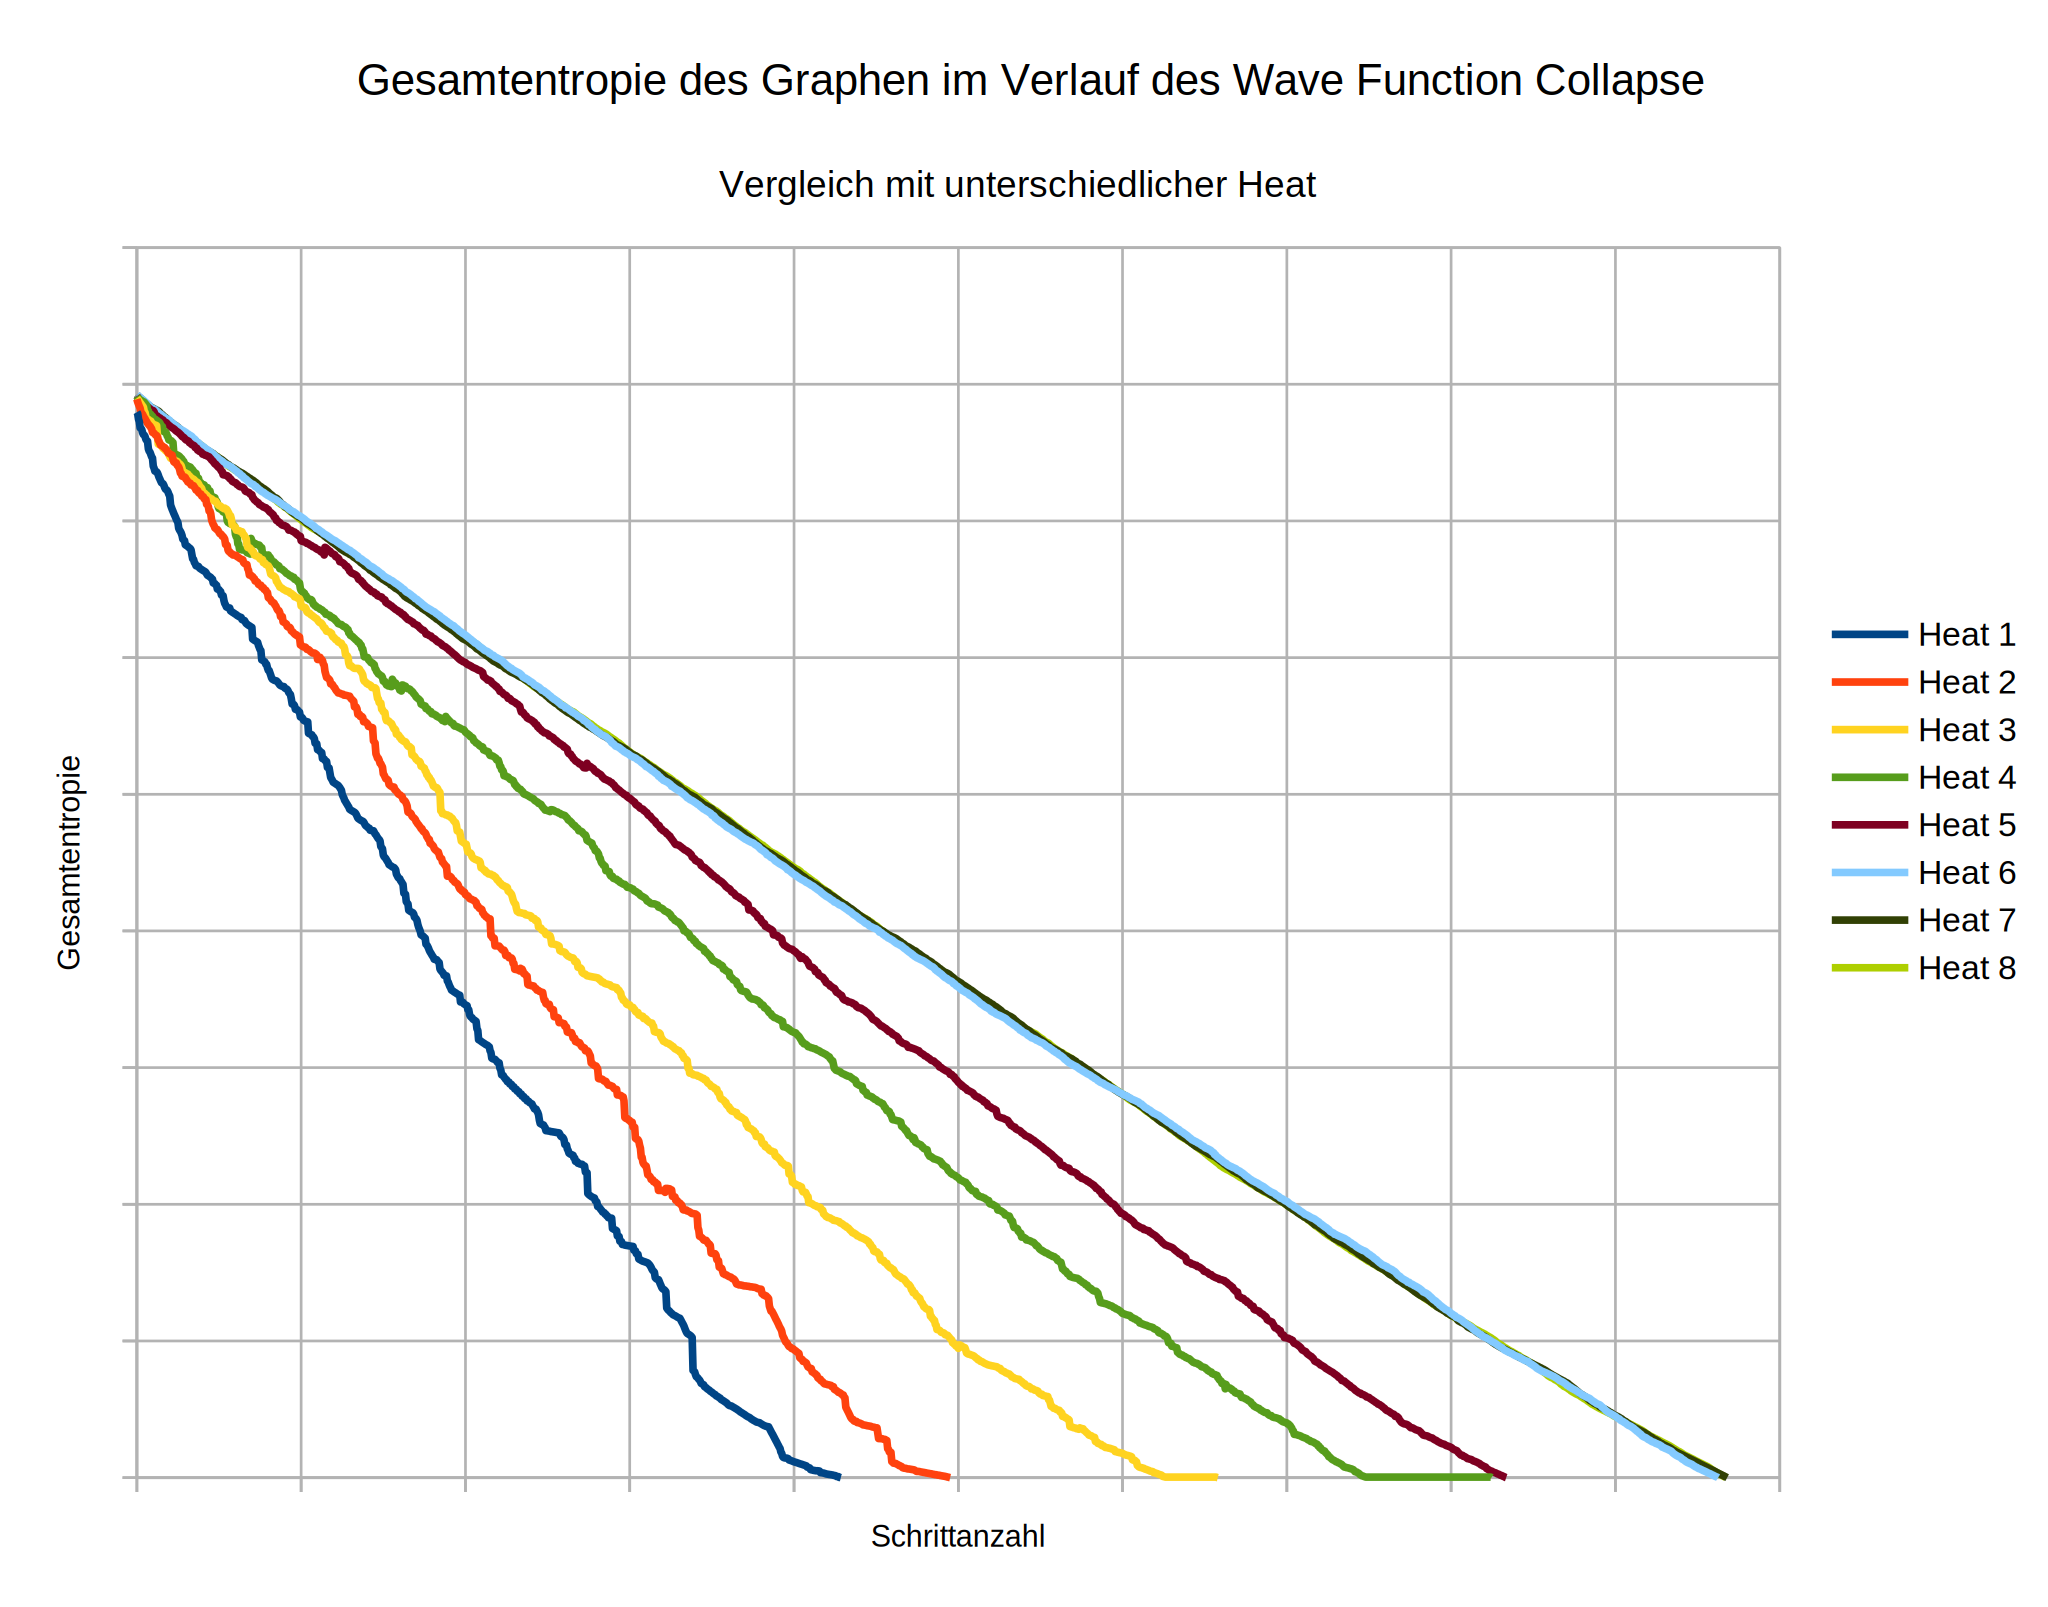
\includegraphics[width=\linewidth]{data/voronoi_clipping/1.png}
        \caption{}
    \end{subfigure}\hfill
    \begin{subfigure}{0.32\textwidth}
        \centering
        \includegraphics[width=\linewidth]{data/voronoi_clipping/2.png}
        \caption{}
    \end{subfigure}\hfill
    \begin{subfigure}{0.32\textwidth}
        \centering
        \includegraphics[width=\linewidth]{data/voronoi_clipping/3.png}
        \caption{}
    \end{subfigure}
    
    \vspace{4mm}
    
    \begin{subfigure}{0.32\textwidth}
        \centering
        \includegraphics[width=\linewidth]{data/voronoi_clipping/4.png}
        \caption{}
    \end{subfigure}\hfill
    \begin{subfigure}{0.32\textwidth}
        \centering
        \includegraphics[width=\linewidth]{data/voronoi_clipping/5.png}
        \caption{}
    \end{subfigure}\hfill
    \begin{subfigure}{0.32\textwidth}
        \centering
        \includegraphics[width=\linewidth]{data/voronoi_clipping/6.png}
        \caption{}
    \end{subfigure}
    
    \caption{
        Voronoizellen auf gewünschten Bereich zuschneiden
        \\(a) Die Voronoizelle ragt über den Bereich hinaus
        \\(b) Ersetze den Eckpunkt außerhalb des Bereichs mit den Schnittpunkt der Kante zum Bereichsrand
        \\(c) Der nächste Schnittpunkt mit der linken Seite des Bereichs liegt außerhalb 
        \\(d) Finde einen besseren Schnittpunkt entlang des anderen Rands
        \\(e) Der nächste Schnittpunkt liegt auf dem Eckpunkt der Kante und entfällt
        \\(f) Nach beschneiden der letzen Kante erhalten wir eine korrigierte Voronoizelle
    }
    \label{fig:voronoi_clipping}
\end{figure}



\subsection{Collapse Cells - Step}

\at{@placement} Ein Schritt besteht aus Search, Pick, Collapse und Propagate Phase.

\begin{enumerate}
    \item Search: ermittle alle Zellen mit der geringsten Entropie (Shannon - Entropie) die noch nicht Collapsed ist
    \item Pick: wähle eine der gefundenen Zellen
    \item Collapse: wähle aus der Menge an noch möglichen Zuständen einen aus, skalierte Chance basiert auf dessen Frequenz in der Eingabe
    \item Propagate: Keep a list of cells that changed. Add the collapsed cell onto the list. Then until its empty:
    \subitem Pop off a changed cell and for each of its neighbours recalculate their set of possible states. If any state became impossible, append that neighbour onto the list. If any neighbour now has no more possible states we reached a contradiction.
\end{enumerate}

If we can collapse all cells then we found a valid solution for the given input pattern and graph. Otherwise we reached a contradiction, when at least one cell could no longer be collapsed into a single state.
To handle a contradiction, we need to trace back to an early stage of the collapse and make a different decision, in hope that from there we can reach a solution (\@todo(viktor):{ provability of a solve and NP-Hardness}). The points at which the algorithm ''decides'' are when Picking a cell with the lowest entropy and when Collapsing a cell into any one of its possible states. If we do not want to store any of the intermediates states of the graph, we can just go back to the first decision point, when the grid was just initialized. In other words, we just restart and try again. Otherwise we can also store some information to allow us to return to a partially solved version of the graph.



\subsection{Backtracking}
Wenn der Algorithmus einen Widerspruch entdeckt, muss nicht immer alle Arbeit verworfen werden. Gerade bei größeren oder komplizierteren Mustern oder Graphen ist es wahrscheinlich, dass beim ersten Versuch keine Lösung gefunden wird, weil die Komplexität den Lösungsraum stärker einschränkt. Wenn ein Widerspruch in einer Zelle aber nun nur von den direkten Nachbar abhängt, so ist es wahrscheinlich dass weiter entfernte bereits gelöste Zellen dennoch kompatibel sind. Um einen lokalen Widerspruch aufzulösen muss meistens nur lokal eine andere Entscheidung getroffen werden.

Um Backtracking umzusetzen müssen mehr Informationen behalten werden als nur der Zustand des Gitters zum aktuellen Zeitpunkt. Will man nun wieder einen Schritt zurückgehen muss man wissen, welche Entscheidung man zuvor bereits getroffen hat um dessen Effekt rückgängig zu machen. Dabei genügt es nicht nur die Collapste Zelle und den Zustand wieder zu entfernen, weil jede Zelle von mehreren Nachbarn beeinflusst wird. Die Zustandsmenge einer Zelle ist die Schnittmenge der möglichen Nachbarzuständen der Nachbar. Somit kann es sein, dass ein Zustand A aus der Menge wegen mehreren Einschränkungen von mehreren Nachbarn fehlt. Nimmt man nun durch Backtracking eine dieser Einschränkungen wieder zurück, so ist es nicht offensichtlich, ob Zustand A nun wieder möglich ist, ohne alle Einschränkungen auf die Zelle neu zu berechnen.
Entweder man macht die Änderung nur lokal rückgängig und berechnet immer alle Zellen neu, bis sich keine mehr ändern. Oder man speichert ab, zu welchem Zeitpunkt ein Zustand unmöglich geworden ist und prüft ob dieser Zeitpunkt nach dem Schritt zurück weiterhin in der Vergangenheit oder nun in der Zukunft liegt. Bei zweiterem müssen alle solche Zustände als wieder möglich betrachtet werden.
Diese Art die Menge an Zuständen darzustellen ist gut, weil sich für jede Zelle die Zustandsmenge in jedem Schritt des Algorithmus immer nur verkleinert oder gleichbleibt. Ist ein Zustand durch die Nachbar unmöglich so wird er auch nie wieder an späterem Zeitpunkt möglich.

Desweiteren wollen wir bereits gemachte Entscheidungen nicht noch einmal wiederholen, wenn diese zu einem Widerspruch führen werden. Die Entscheidungspunkte in der  Pick und Collapse Phase können gleich behandelt werden. Wir können die List an Auswahlmöglichkeiten für später speichern und die ausgewählte Zelle oder den ausgewählten Zustand von der Liste entfernen. Kommen wir nun zu diesem Schritt zurück können wir einfach die nächste Möglichkeit auswählen und den Algorithmus normal weiterlaufen lassen.

\@todo(viktor):{ Pseudo-Code oder Diagramme für Algorithmus and Backtracking?}

In der Umsetzung speichere ich für jede Zelle eine Liste aller Zustände. Jeder Zustand ist entweder möglich und wurde noch nicht entfernt oder ist unmöglich und speichert den Zeitpunkt an dem er unmöglich wurde. Hierbei ist der Zeitpunkt einfach die Anzahl an Schritten des Algorithmus. 
Für jeden Schritt des Algorithmus speichern wir nun die Liste der gefundenen Zellen in Search. Wenn in Pick eine Zelle ausgewählt wird, entfernen wir diese aus der Liste und wählen beim Backtracken nun eine andere. Ebenso speichern wir vor der Collapse Phase alle wählbaren Zustände und entfernen mit jedem Lösungsversuch den gewählten Zustand. 

Nun haben wir unwissentlich auch eine Schwachstelle in den Algorithmus eingeführt. Wenn wir zuvor in der Search-Phase keine Zellen in Superposition mehr gefunden haben, waren alle Zellen tatsächlich collapsed. Nun kann es auch sein, dass alle Zellen, die wir finden, zu einem Widerspruch führen. Auch in der Collapse-Phase war es unmöglich keinen Zustand mehr auswählen zu können, da eine Zelle mit leerer Zustandmenge bereits zuvor als Widerspruch identifiziert wurden wäre. 
Um diese Fälle ordentlich zu behandeln können wir nun aber einfach auch in solchen Fällen einen Widerspruch deklarieren und Backtracken. Schließlich haben wir alle noch möglichen Entscheidungen bereits getroffen und ausgewertet und keine Lösung gefunden. Somit führt dieser Schritt zwar nicht direkt zu einem Widerspruch in einer Zelle, aber alle folgen Schritte werden irgendwann zu einem Widerspruch führen. Zu Bemerken ist, dass wenn auf diese Weise bis zum ersten Schritt gebacktrackt wird und auch die erste Entscheidung einen Widerspruch verursacht, so kann die Kombination aus Eingabe und Graph keine Ausgabe ergeben.


\subsection{Overlap - Direction Mask / State Buckets / rule sets}
\begin{itemize}
    \item \@todo(viktor):{ Strictness muss ich nicht mit der Größe der Zahl im Code hier gleichstellen, dass ist nur verwirrend wenn 'hohe' strictness eigentlich weniger strenge bedingungen darstellt}
    \item Da Nachbarn nun in beliebigen Richtungen zu finden sind, gibt es kein direktes mapping zu den Supportregeln, welche ja je eine Menge pro Richtung sind.
    \item Dabei können wir entscheiden ob jeweils nur eine Menge oder mehrere Mengen betrachtet werden
    \item Ob eine Menge erlaubt ist, messen wir indem wir berechnen wir nahe die tatsächliche Richtung zu den Mengenrichtungen ist. Nun wählen wir die x-nähesten Mengen aus. Bei einer Strenge von 1 also die beste, bei 2 die zwei besten und so weiter.
    \item Die Strenge kann maximal 8 betrangen, da wir nur 8 "Himmelsrichtungen`` in der Extraktion genutzt haben. 
    \item Insgesamt bedeutet dies, dass ein Nachbar als z.B. im Norden oder im Nordosten betrachtet werden kann. Dadurch ist die menge an kompatiblen zuständen weniger eingeschränkt und es ist weniger wahrscheinlich, dass alle Zustände einer Zelle unmöglich werden
    \item Es folgt aber auch, dass nun Nachbar mit fast oder gar perfekter \\ übereinstimmung mit einer der Himmelsrichtung als nicht nur diese gelten, wodurch es zu einer Verzerrung im Output kommt.
    \item Wenn zuvor ein Muster im Input z.B. stehts N-S ausgerichtet war kann es ab einer Strenge vom 3 auch als (NW, N, NO)-(SW, S, SO) betrachtet werden. es könnte also auch als NW-SW betrachtet werden und aus einem Geradlinigen muster wird ein geknicktes oder zackiges.
    \item Aber genau diese auflockerung ist nötig, damit der Algorithmus mit \\ höherer Wahrscheinlichkeit eine Lösung findet
    \item 
    \item Wenn mehr Richtungen erlaubt sind, so kann dies auch betrachtet werden als dass nun nicht nur das Eingabe Muster sondern auch gedrehte Versionen der Eingabe möglich sind. 
    \item Nun können gedrehte regelmäßige Gitter auch gelöst werden. (Siehe Grid = Square with an angle ~27° and strictness(\at{@naming}) 1 or 2).
    \item Auf unregelmäßigen Gittern kann man keine Drehung finden in der es einem regelmäßigen Gitter global gleich. Dennoch können Lösungen gefunden werden, da für jedes Zellenpaar/Benachbarung frei gewählt werden kann, ob eine solche gedacht Drehung angewendet wird oder nicht. 
    \item Es ist so, als würde der Algorithmus das Gitter lokal immer genau so verdrehen (mit Beschränkung durch die maximal Strictness), dass das tatsächliche Gitter lokal einem regelmäßigen gleicht.
    \item 
    \item Bei höherer Strictness und einer gelösten Zelle: ein Nachbar der Zelle kann nun aus mehr als einer Regelmenge entsprechend seiner Richtung wählen. Die Superposition des Nachbarn ist 'größer' bei höherer Strictness. Dadurch ist auch die Menge an Zuständen die Nachbarn des Nachbarn haben entsprechend größer, da weniger Beschränkungen auf sie einwirken. Es bleiben für einen längeren Zeitraum mehr Zustände möglich, wodurch ein Widerspruch durch eine Zelle mit leerer Superposition weniger wahrscheinlich ist. Im Gegenzug ist die lokale Ähnlichkeit zum Original verringert, da nun auch Nachbarn mit 'eindeutiger' Richtung zur Zelle auch einer weniger passenden Richtung zugewiesen werden können.
    \item Eine globale Strictness für alle Zellen hat einen negativen Effekt auf lokal regelmäßige Regionen eines Gitters und ein postiven Effekt auf sehr unregelmäßige Regionen des Gitters.
    \item Anstatt dass die Strictness global für alle Zellen zu Beginn bestimmt wird, kann man auch während des Collapse 'lernen' welche Regionen 'schwerer' zu lösen sind und dort die Strictness schrittweise erhöhen bis eine Lösung gefunden werden kann.
\end{itemize}